\chapter{Ergebnisse}

\section{Python-Interface f"ur MCTDH}
\label{sec:PyInterface}


Es wurde eine Programmierschnittstelle (von englisch \textit{application programming interface}, API) f"ur das MCTDH-Programmpaket erstellt.
Im Rahmen dieser Arbeit wurde sich auf Klassen beschr"ankt, welche f"ur das Einlesen der baumf"ormig strukturierten MCTDH-Basis zust"andig sind.
Die Klassen und Methoden, die "uber Python aufgerufen werden k"onnen, sind in Abbildung \ref{fig:uml_Cython} dargestellt. 
Jede Klasse der API wird in Abbildung \ref{fig:uml_Cython} durch einen Kasten repr"asentiert. Im oberen Teil des Kastens ist der Klassenname
angegeben und im unteren Teil sind die Methoden der Klasse aufgelistet. Die Anordnung der K"asten gibt die Abh"angigkeit der Klassen zueinander wieder.
So muss ein Objekte von der Klasse \textit{ControlParameter} generiert werden, um Objekte der Klasse
\textit{mctdhBasis} erzeugen zu k"onnen. Analog h"angen die Klassen \textit{Tdim} und \textit{physCoor} von der Klasse \textit{mctdhNode} ab.
\textit{ControlParameter} und \textit{mctdhBasis} sind die Klassen, die die Konfigurations- und Basisdatei einlesen
und die Genauigkeitsparameter und die MCTDH-Basis verwalten. Dagegen wird in der Klasse \textit{mctdhNode} die lokale Information
eines Knotens verwaltet.
So  k"onnen Knoteneigenschaften "uber die Klasse \textit{mctdhNode} ermittelt werden. 
Die Knotenobjekte k"onnen in Nachbarknoten "uberf"uhrt werden.
Die SPFs eines Knoten wird in der Klasse \textit{Tdim} ermittelt. Mit der Klassen \textit{physCoor} k"onnen
die Schwingungsmoden, der untersten Knoten bestimmt werden. 

Zur Demostration der API wird im folgenden ein Python-Skript vorgestellt, mithilfe dessen die Gr"o"se einer MCTDH-Wellenfunktion berechnet wird:

\newpage

\begin{verbatim}
    import mctdh

    config = mctdh.controlParameters()
    config.initialize('mctdh.config')
    basis = mctdh.MctdhBasis()
    basis.initialize('basis.txt', config)
    
    maxNodes = basis.NmctdhNodes()
    
    nodes_spf = {}
    for i in range(maxNodes):
        node = basis.MCTDHnode(i)
        tdim = node.t_dim()
        nodes_spf[i] = tdim.GetnTensor() 
    
    primitivB = {i: basis.MCTDHnode(i).t_dim().active(0) for i in \
                range(maxNodes) if \
                basis.MCTDHnode(i).Bottomlayer() == True
    ProdBottomNode = {}
    for key in primitivB:
        ProdBottomNode[key] = primitivB[key] * nodes_spf[key]
    ProdBottom = sum([l_[1] for l_ in ProdBottomNode.items()])

    print ProdBottom

    TopNode = 0
    for i in range(maxNodes):
        if basis.MCTDHnode(i).Toplayer() == True:
                children = basis.MCTDHnode(i).NChildren()
                for j in range(children):
                    TopNode *= basis.MCTDHnode(i).down(j).t_dim().GetnTensor()
                TopNode *= basis.MCTDHnode(i).t_dim().GetnTensor()

    print TopNode
    
    remnantNodeList = []
    remnant = 0
    for i in range(maxNodes):
        if basis.MCTDHnode(i).Toplayer() == False and \
        basis.MCTDHnode(i).Bottomlayer() == False:
                children = basis.MCTDHnode(i).NChildren()
                parent = basis.MCTDHnode(i).t_dim().GetnTensor()
                for j in range(children):
                    remnant *= basis.MCTDHnode(i).down(j).t_dim().GetnTensor() 
                remnant *= parent
                remnantNodeList.append(remnant)
                remnant = 0
    remnantSum = sum(remnantNodeList)
    
    print remnantSum
    
\end{verbatim}


Die in Abbildung \ref{fig:uml_Cython} dargestellte Klassen k"onnen mit folgenden Befehl in Python aufgerufen werden:

\begin{verbatim}
import mctdh
\end{verbatim}

Um in Python die MCTDH-Klassen verwenden zu k"onnen, gen"ugt es \textit{mctdh} dem Klassennamen voranzustellen und durch einen
Punkt zu trennen.

\begin{verbatim}
config = mctdh.controlParameters()
basis = mctdh.MctdhBasis()
\end{verbatim}

"Uber die initialisierten Objekte kann auf die Klassenmethoden zugegriffen werden: 
\begin{verbatim}
config.initialize('mctdh.config')
basis.initialize('basis.txt', config)
\end{verbatim}

Mithilfe des Objektes \textit{basis} kann die Anzahl der Knoten des eingelesenen MCTDH-Baums bestimmt werden:
\begin{verbatim}
maxNodes = basis.NmctdhNodes()
\end{verbatim}

Um die Gr"o"se der Wellenfunktion berechnen zuk"onnen, wird die Anzahl der SPFs eines Knotens
und die Anzahl der SPFs aller Nachbarknoten multipliziert.
Alle SPFs werden in den Dictionary-Datentyp \textit{nodes\_spf} gespeichert. 
Anschlie"send wird die Summe aller SPFs-Produkte gebildet.
Hierf"ur werden die Summen der Produkte vom oberen Knoten, von den unteren Knoten und von denen
restlichen Knoten separat gebildet und in einem Dictionary bzw. einer Liste gespeichert:

\begin{verbatim}
nodes_spf = {}
ProdBottomNode = {}
remnantNodeList = []
\end{verbatim}

Der Datentyp Dictionary wird mit geschweiften Klammern und der 
Datentyp Liste wird mit eckigen Klammern deklariert.
Die Berechnung der Gr"o"se der Wellenfunktion wird in einer Funktion vorgenommen:

\begin{verbatim}
def get_SPFs()
\end{verbatim}

Die Anzahl der SPFs und primitiven Basis werden jeweils in verschiedene Dictionaries gespei\-chert:

\begin{verbatim}
for i in range(maxNodes):
    node = basis.MCTDHnode(i)
    tdim = node.t_dim()
    nodes_spf[i] = tdim.GetnTensor() 

primitivB = {i: basis.MCTDHnode(i).t_dim().active(0) for i in \
            range(maxNodes) if \
            basis.MCTDHnode(i).Bottomlayer() == True}
\end{verbatim}

In der for-Schleife werden alle Knoten des Baums erfasst und f"ur jeden i-ten Knoten 
wird die Anzahl an SPFs in \textit{nodes\_spf} gespeichert.
Die Anzahl der primitiven Basis wird in dem Dictionary \textit{primitivB} gespeichert.
Dabei wird "uber alle Knoten iteriert, die zu den untersten Knoten geh"oren und
die Gr"o"se der primitiven Basis wird mit \textit{active(0)} im Dictionary mit dem Index
$i$ gespeichert.
Die Anzahl der SPFs und der primitiven Basis der untersten Knoten wird f"ur jeden Knoten
multipliziert.
Anschlie"send werden die Produkte summiert und die Summe in textit{ProdBottom} gespeichert:

\begin{verbatim}
for key in primitivB:
    ProdBottomNode[key] = primitivB[key] * nodes_spf[key]
ProdBottom = sum([l_[1] for l_ in ProdBottomNode.items()])
\end{verbatim}

Die for-Schleife iteriert "uber alle Indizes des Dictionary \textit{primitivB}.
Da die untersten Knoten in \textit{primitivB} dieselben Indizes besitzen, ist
gew"ahrleistet, dass nur Produkte aus der Anzahle der SPFs und der primitven Basis 
f"ur jeden untersten Knoten berechnet werden.

Das Produkt aus SPF-Anzahl des ersten Knoten und seiner Nachbarknoten wird im folgenden
Code-Abschnitt berechnet:

\begin{verbatim}
for i in range(maxNodes):
    if basis.MCTDHnode(i).Toplayer() == True:
            children = basis.MCTDHnode(i).NChildren()
            for j in range(children):
                TopNode *= basis.MCTDHnode(i).down(j).t_dim().GetnTensor()
            TopNode *= basis.MCTDHnode(i).t_dim().GetnTensor()
\end{verbatim}

Zun"achst wird die Anzahl an Nachbarknoten berechnet und in der Variabel \textit{children} gespeichert.
Es wird "uber alle Nachbarn iteriert und das Produkt der SPF-Basisgr"o"se aller Nachbarknoten
 und des obersten Knoten gebildet und in TopNode gespeichert.

Im letzten Code-Block wird die Summe aus den restlichen Produkten gebildet:

\begin{verbatim}
for i in range(maxNodes):
        if basis.MCTDHnode(i).Toplayer() == False and \
        basis.MCTDHnode(i).Bottomlayer() == False:
                children = basis.MCTDHnode(i).NChildren()
                parent = basis.MCTDHnode(i).t_dim().GetnTensor()
                for j in range(children):
                    remnant *= basis.MCTDHnode(i).down(j).t_dim().GetnTensor() 
                remnant *= parent
                remnantNodeList.append(remnant)
                remnant = 0
    remnantSum = sum(remnantNodeList)
\end{verbatim}

Es wird "uber die restlichen Knoten iteriert, die Nachbarknoten werden bestimmt und die Produkte
der Basisgr"o"sen werden gebildet und in der Liste \textit{remnantNodeList} gespeichert.
Die Addition der Produkte aus den obersten, untersten und restlichen Knoten ergibt die
Gr"o"se der Wellenfunktion, die von der Funktion zur"uckgegeben wird: 

\begin{verbatim}
 return ProdBottom + TopNode + remnantSum
\end{verbatim}

Durch den \textit{print}-Befehl wird das Ergebnis der Funktion ausgegeben:

\begin{verbatim}
print get_SPFs()
\end{verbatim}
    
\begin{figure}
    \centering
    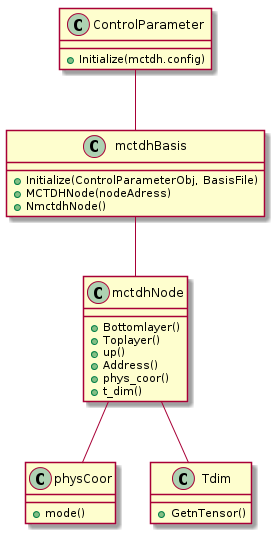
\includegraphics[scale=0.6]{figures/sequenceDiagram}
    \caption{Alle Klassen, die in Cython erstellt wurden, sind mit einem ,,C'' gekennzeichnet. Die jeweiligen Klassenmethoden sind mit einem
    gr"unen Punkt gekennzeichnet.}\label{fig:uml_Cython}
\end{figure}








\section{Graphische Benutzeroberfl"ache f"ur MCTDH}

Zur Demonstration der graphischen Benutzeroberfl"ache wird im folgenden das Vorgehen zum Starten einer 
MCTDH Simulation vorgef"uhrt. Als Beispiel dient die Photodissociation von NOCl.

\begin{figure}
    \centering
    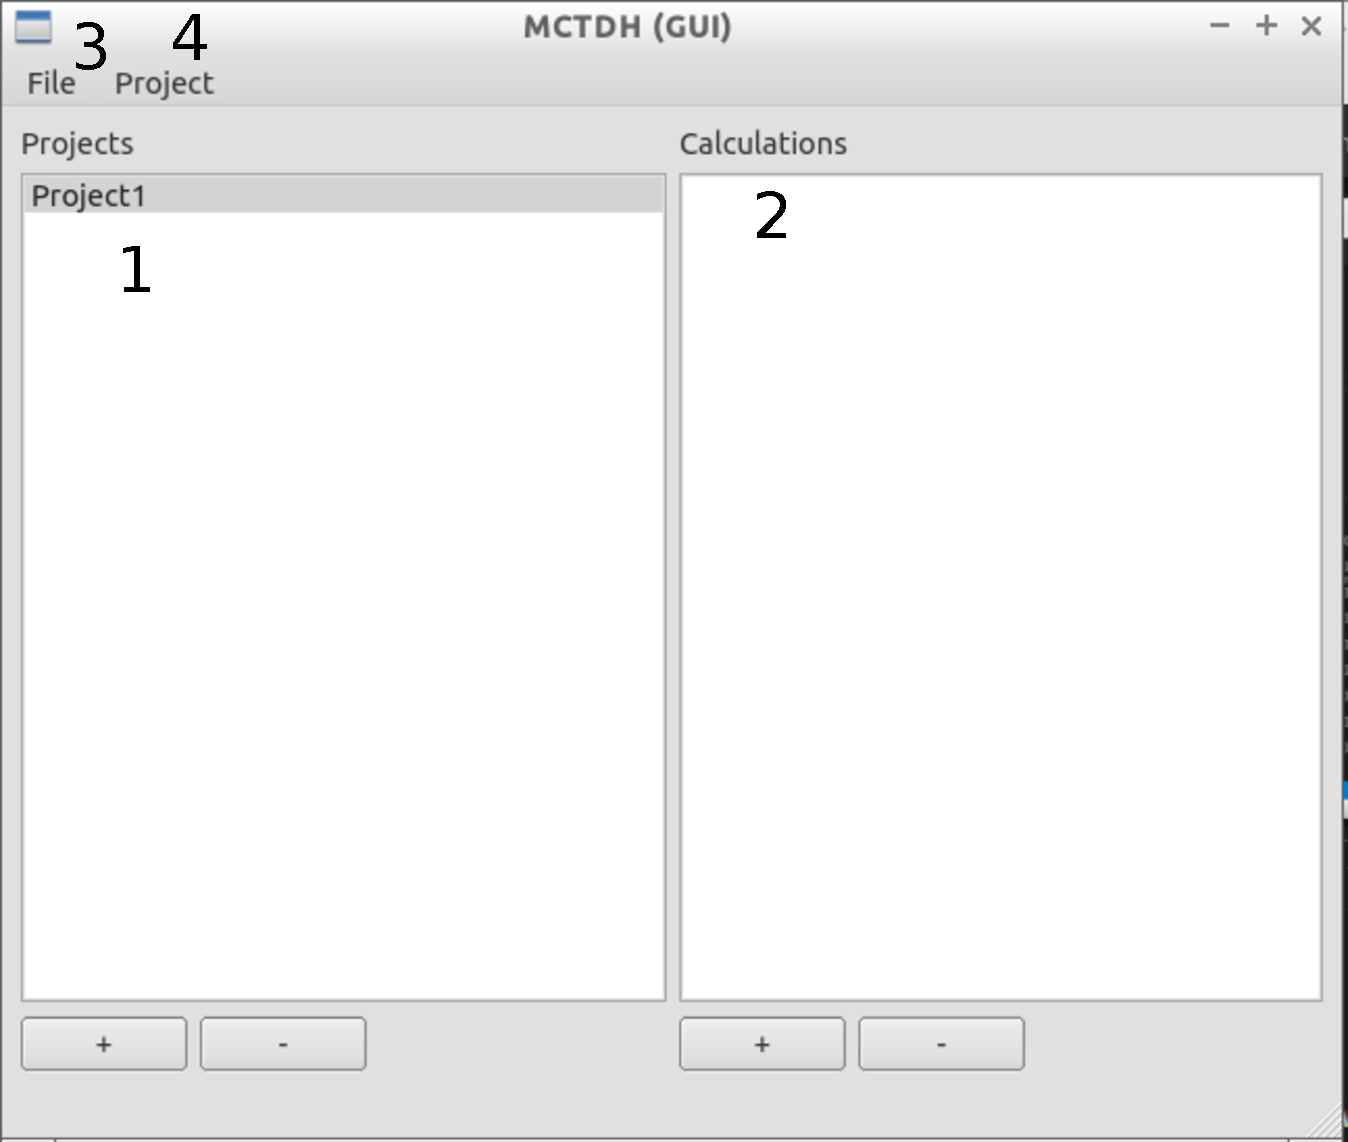
\includegraphics[scale=0.5]{figures/screenMain}
    \caption{Hauptfenster der MCTDH-GUI}\label{fig:workflow1}
\end{figure}

Bei Start der GUI erscheint das Hauptfenster (siehe Abbildung \ref{fig:workflow1}).
In Liste \textbf{1} sind alle vorhandenen Projekte aufgef"uhrt.
Nach Auswahl eines Projekts erscheinen in Liste \textbf{2} alle dem Projekt zugeorednete Rechnungen.
Durch die Schaltfl"achen ,,+'' und ,,-'' k"onnen Projekte sowie Rechnungen jeweils hinzugef"ugt bzw.
entfernt werde.
Im ,,File'' \textbf{3} befinden sich zus"atzliche Optionen zur Projektverwaltung (siehe Abbildung \ref{fig:workflow2}).
Durch Klicken der Schaltfl"ache \textbf{5} wird ein neues Projekt erstellt. Externe Projekte werden durch die 
Schaltfl"ache \textbf{6} geladen. Bet"atigung der Schaltfl"ache \textbf{7} beendet die Benutzeroberfl"ache.

\begin{figure}
    \centering
    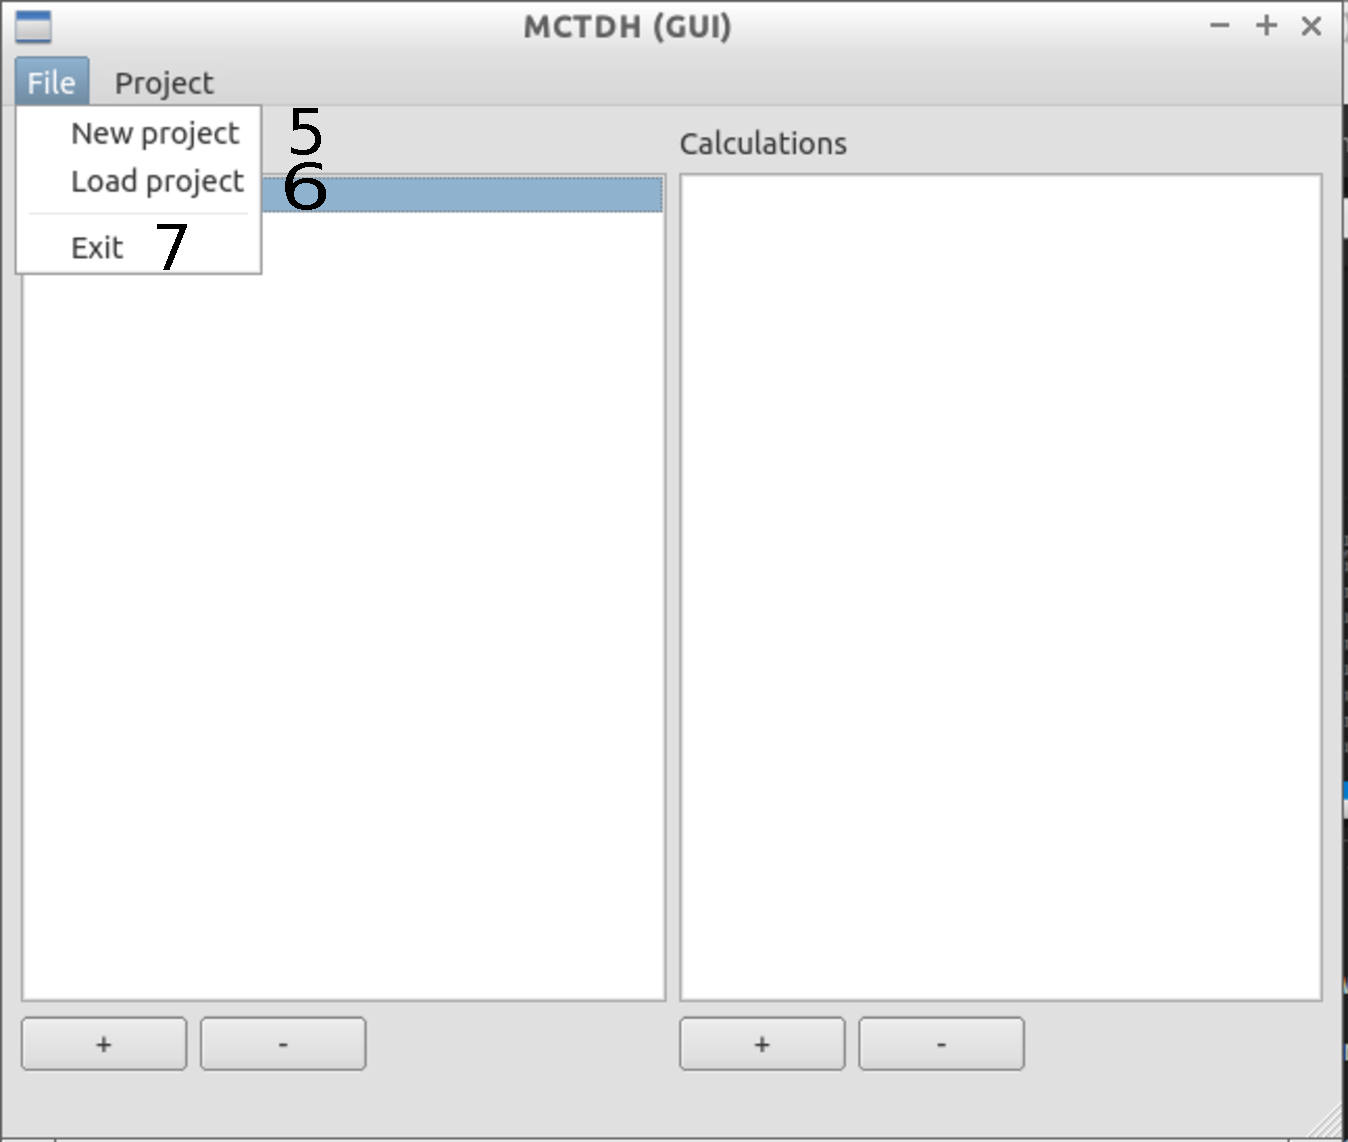
\includegraphics[scale=0.5]{figures/screenMainFile}
    \caption{File-Men"u des Hauptfenster der MCTDH-GUI}\label{fig:workflow2}
\end{figure}

Zum Starten einer neuen Rechnung wird zuerst der Reiter "Project" (Abbildung \ref{fig:workflow1} \textbf{4}) 
ausgew"ahlt. Zwei neue Buttons erscheinen (Abbildung \ref{fig:workflow3}). Durch Klicken von \textbf{8} 
erscheint ein neues Fenster ,,MCTDH calculation'' (siehe Abbildung \ref{fig:workflow4}). 
In diesem Fenster wird die neue MCTDH Rechnung spezifiziert.

\begin{figure}
    \centering
    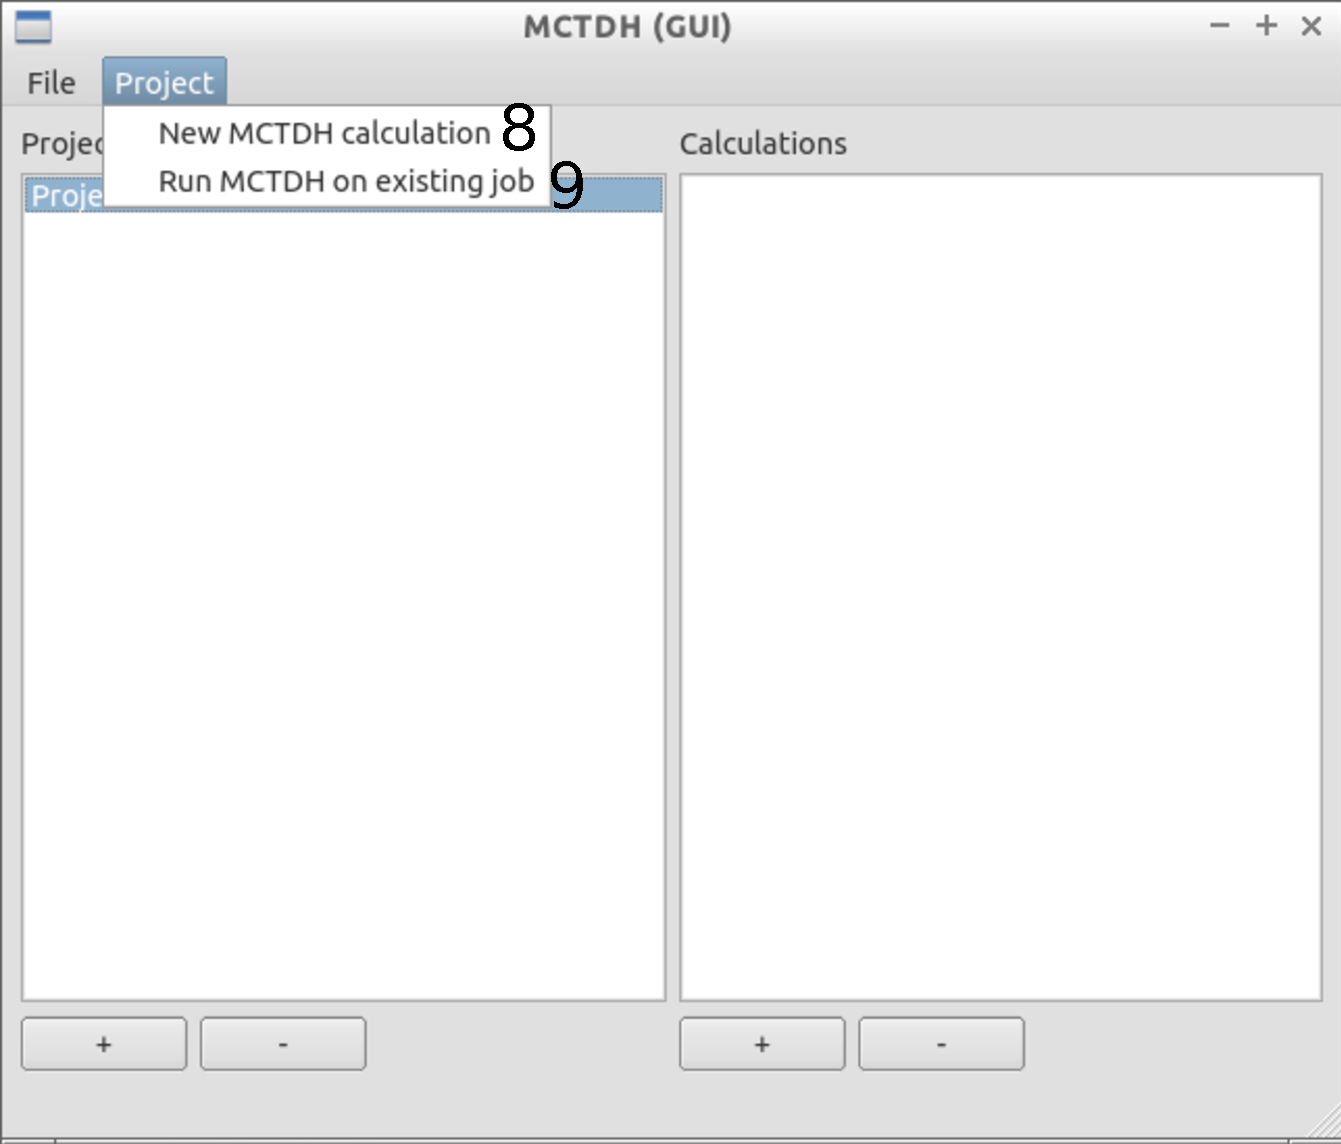
\includegraphics[scale=0.5]{figures/screenMainProject}
    \caption{Eingabefenster der MCTDH-GUI}\label{fig:workflow3}
\end{figure}

In dem Eingabefenster ,,MCTDH calculation'' kann im Feld \textbf{10} der Name der Rechnung angegeben werden. 
Sollte beim Speichern (Abbildung \ref{fig:workflow4} \textbf{18}) des MCTDH-Baums und der Einstellungsparameter 
kein Name angegeben sein, wird der Benutzer 
aufgefordert einen Name f"ur die Rechnung zu w"ahlen. Bevor die Rechnung gespeichert wird, 
wird "uberpr"uft, ob der gew"ahlte Name dem Namen einer andere Rechnung entspricht und, ob diese 
dann gegebenfalls "uberschrieben werden soll.
In Liste \textbf{11} sind verschiedene molekulare Systeme aufgef"uhrt.
"Uber die Kn"opfe \textbf{12} ,,on'' und ,,off''  wird gesteuert, ob eine Potentialfl"ache f"ur die Rechnung verwendet
werden soll. Ist der ,,off'' Knopf aktiviert, werden keine Potentiale in der Liste \textbf{13} angezeigt.
Bei der Standardeinstellung der GUI ist der ,,on''-Knopf aktiviert und es k"onnen Potentiale durch Klicken
auf die Elemente der Liste \textbf{13} ausgew"ahlt werden.
F"ur die MCTDH-Simulation k"onnen vier verschiedene Rechnungen durchgef"uhrt werden \textbf{14}:
Eigenzust"ande, Real- und Imagin"arzeitpropagation und W"armeflusseigenzust"ande.
Des Weiteren kann die Anfangszeit, die Endzeit, die Zeitschritte und die Anzahl an Iterationen f"ur die 
Rechnung angegeben werden \textbf{15}. Alle Parameter werden automatisch geladen, indem eine System aus
Liste \textbf{11} ausgew"ahlt wird oder eine Eingabe-Datei durch 
die ,,Load'' Schaltfl"alche \textbf{19} eingelesen wird. 
Des Weiteren wird der MCTDH-Baum schematisch \textbf{16} als Baumdiagramm angezeigt. 
Zus"atzlich wird der MCTDH-Baum graphisch in \textbf{17} angezeigt. In \textbf{16}
kann durch Doppelklick die Anzahl der SPFs, der primitiven Basis und der Moden ver"andert werden.
Die "Anderung wird instantan im Bild \textbf{17} angezeigt.
Die Schaltfl"ache ,,Cancel'' \textbf{21} beendet das Eingabefenster
und die Schaltfl"ache ,,Start calculation'' \textbf{20} beginnt die MCTDH Simulation.
Alternativ kann die MCTDH Simulation auch aus dem Hauptfenster gestartet werden (siehe Abbildung \ref{fig:workflow3}.
Durch Klicken der Schaltfl"ache ,,Run MCTDH on existing job'' \textbf{9} wird ebenfalls
die MCTDH Simulation gestartet.
In Abbildung \ref{fig:workflow5} wurde das System NOCl geladen, indem auf ,,NOCl'' aus Liste \textbf{11} geklickt wurde.


\begin{figure}
    \centering
    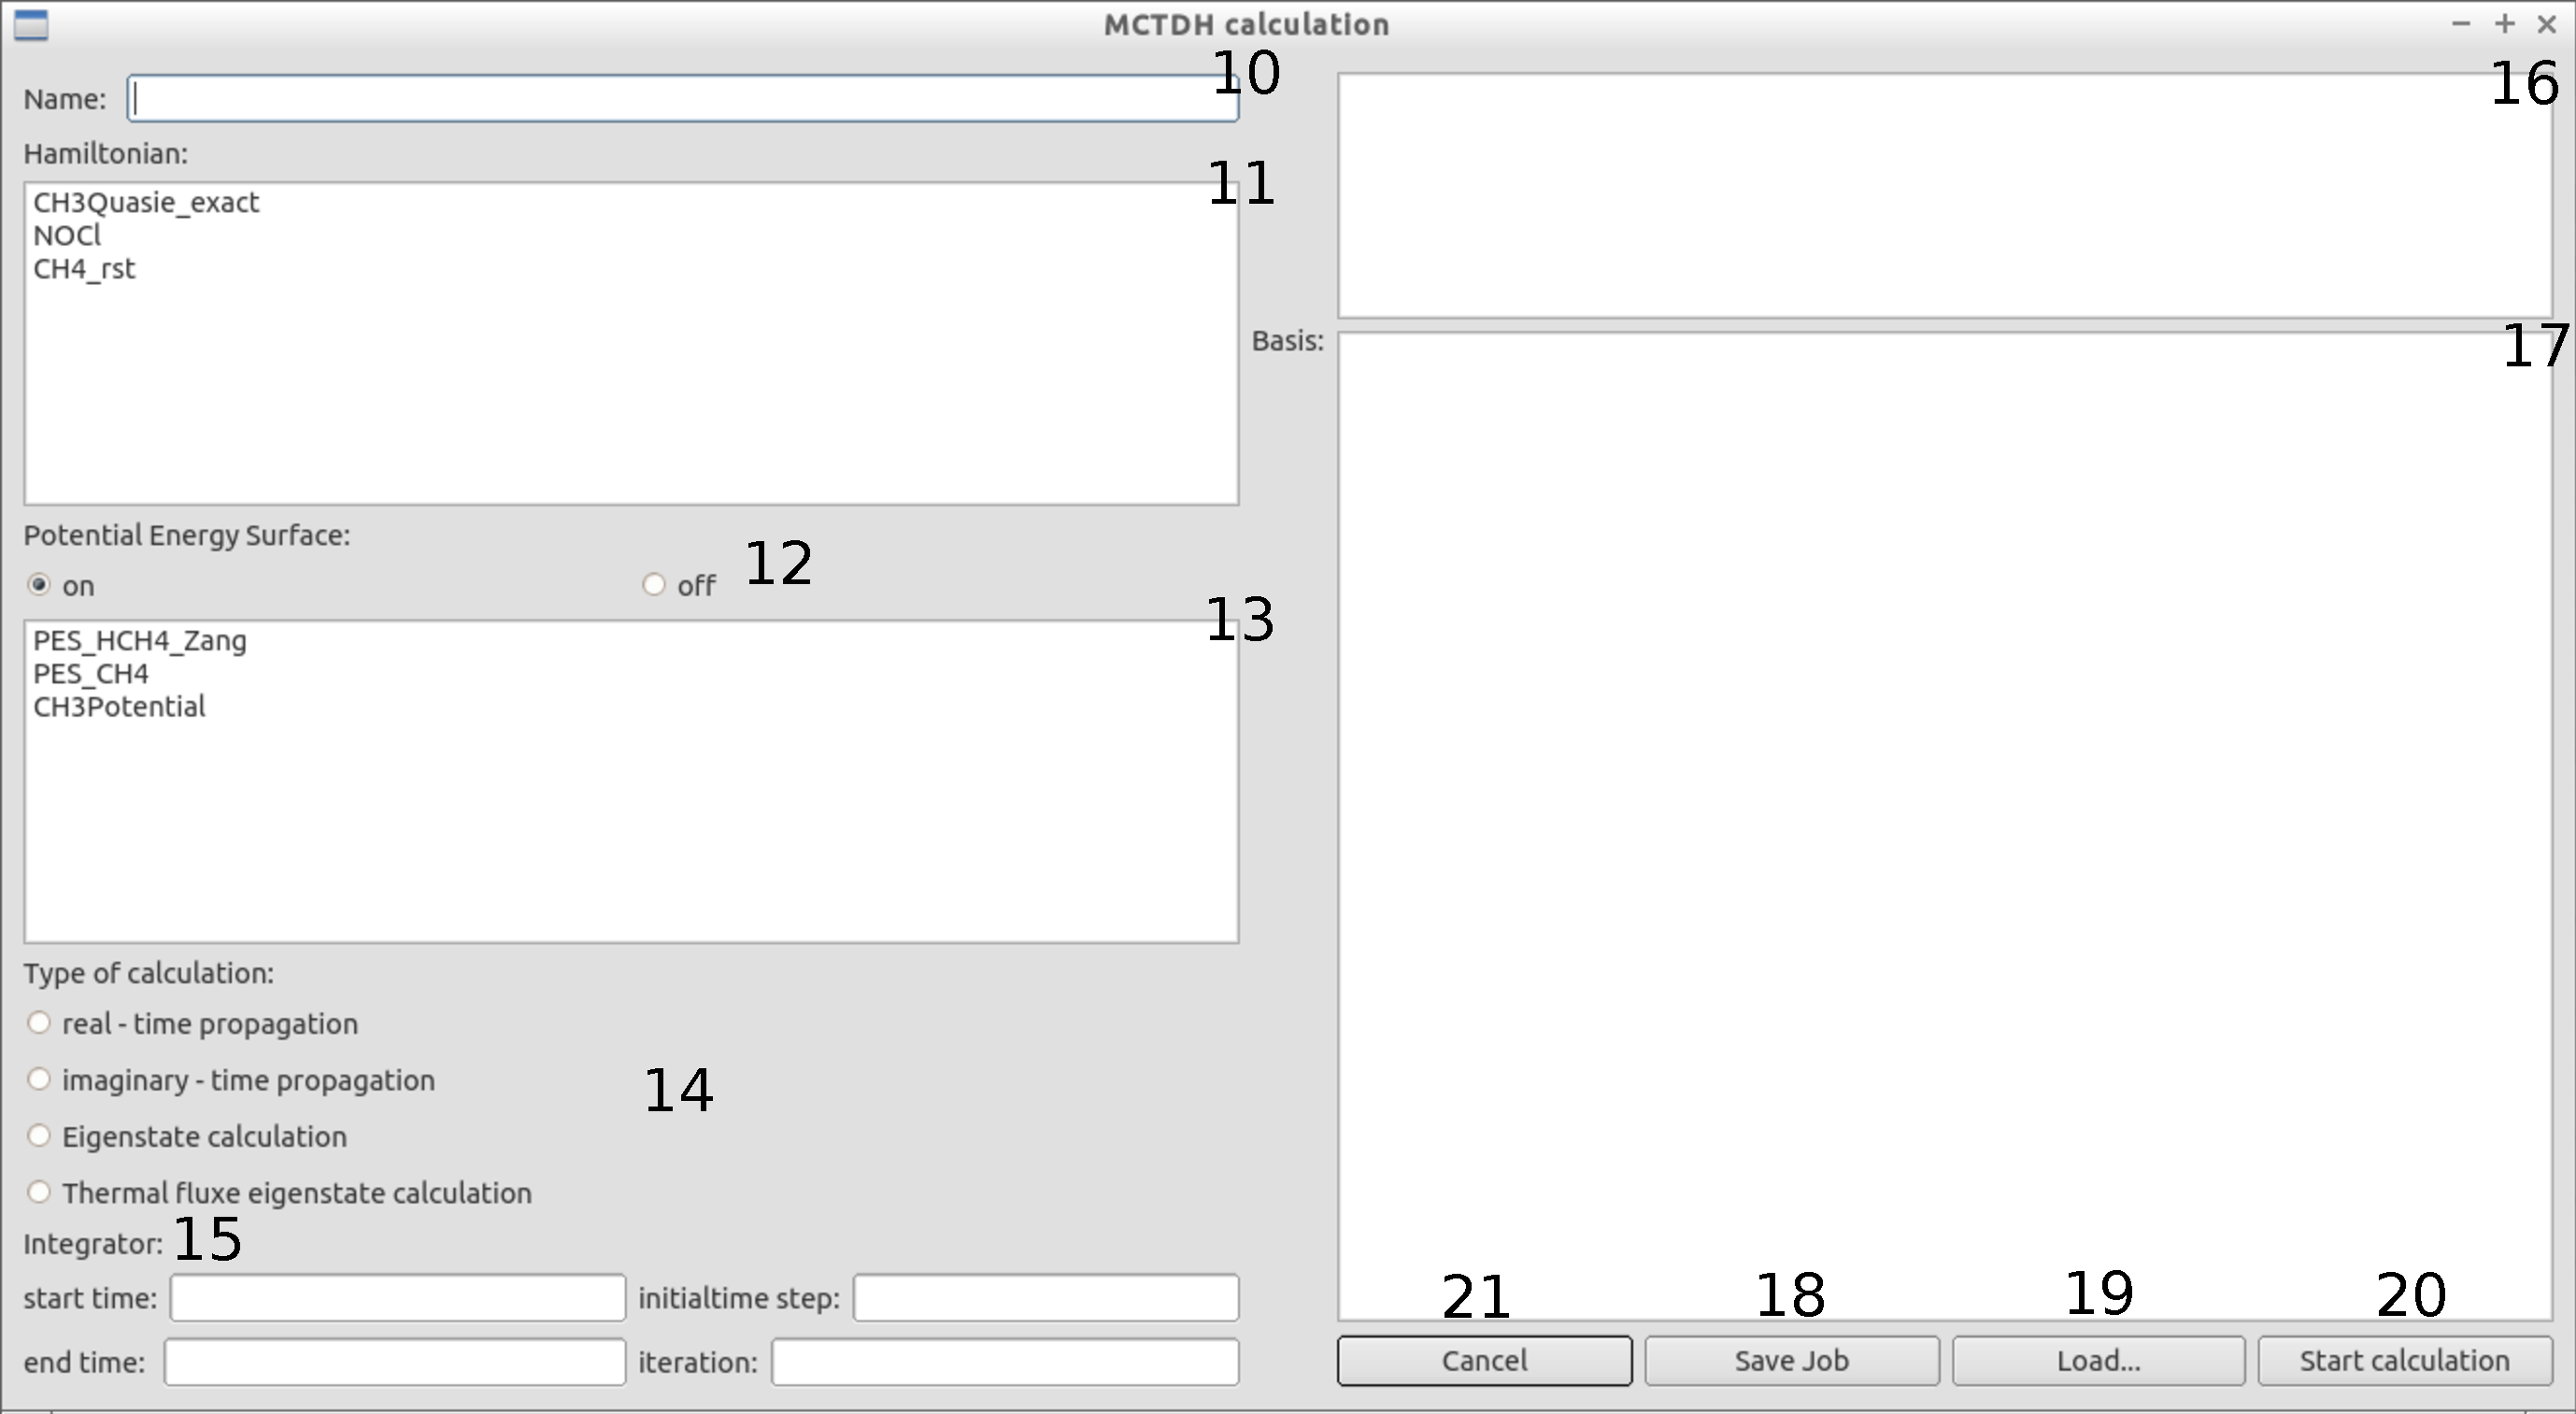
\includegraphics[angle=90, scale=0.45]{figures/screenWidgetA}
    \caption{Eingabefenster der MCTDH-GUI}\label{fig:workflow4}
\end{figure}
\begin{figure}
    \centering
    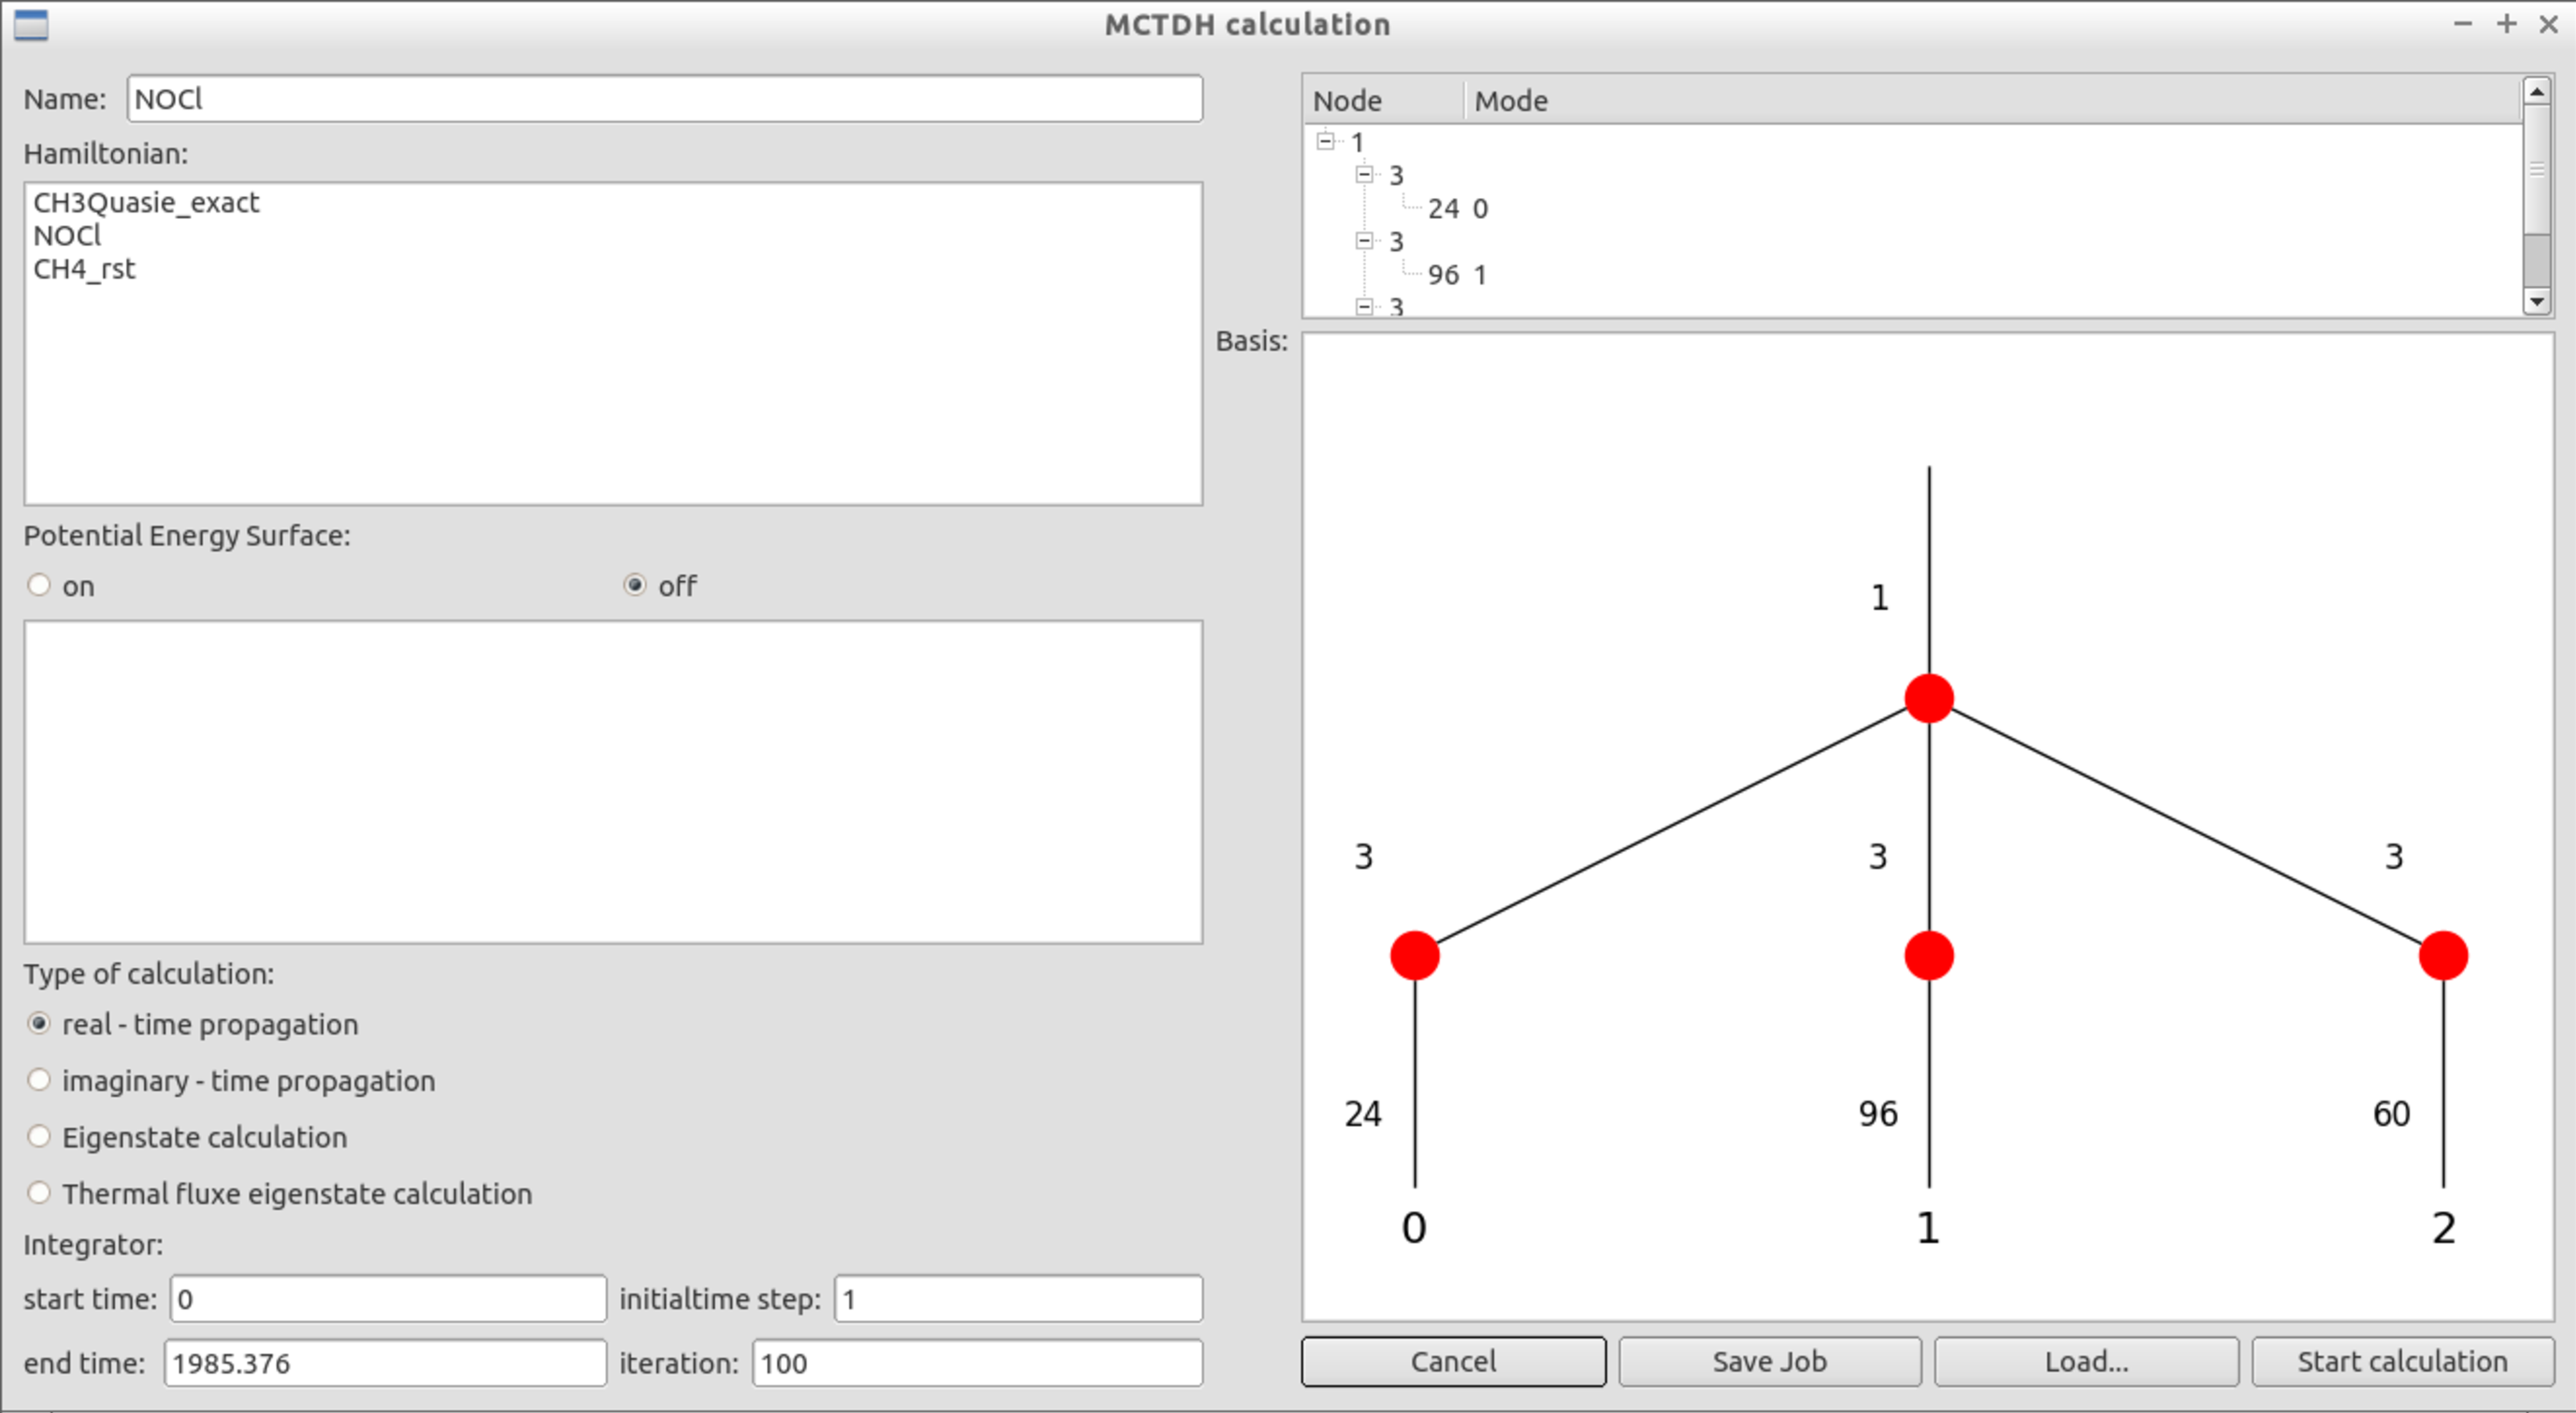
\includegraphics[angle=90, scale=0.45]{figures/screenWidgetAexample}
    \caption{Eingabefenster der MCTDH-GUI am Beispiel der
    Photodissociation von NOCl.}\label{fig:workflow5}
\end{figure}